\documentclass{article}

\usepackage[T1]{fontenc}

\usepackage{fancyhdr} % Required for custom headers
\usepackage{lastpage} % Required to determine the last page for the footer
\usepackage{extramarks} % Required for headers and footers
\usepackage[usenames,dvipsnames]{color} % Required for custom colors
\usepackage{graphicx} % Required to insert images
\usepackage{listings} % Required for insertion of code
\usepackage{courier} % Required for the courier font
\usepackage{lipsum} % Used for inserting dummy 'Lorem ipsum' text into the template
\usepackage{hyperref}
\usepackage{paralist}

% Margins
\topmargin=-0.45in
\evensidemargin=0in
\oddsidemargin=0in
\textwidth=6.5in
\textheight=9.0in
\headsep=0.25in

\linespread{1.1} % Line spacing

% Set up the header and footer
\pagestyle{fancy}
\lhead{\hmwkAuthorName} % Top left header
\chead{\hmwkClass\ (\hmwkClassInstructor): \hmwkTitle} % Top center head
\rhead{\firstxmark} % Top right header
\lfoot{\lastxmark} % Bottom left footer
\cfoot{} % Bottom center footer
\rfoot{Page\ \thepage\ of\ \protect\pageref{LastPage}} % Bottom right footer
\renewcommand\headrulewidth{0.4pt} % Size of the header rule
\renewcommand\footrulewidth{0.4pt} % Size of the footer rule

\setlength\parindent{0pt} % Removes all indentation from paragraphs

\usepackage{listings}
\usepackage{color}

\definecolor{dkgreen}{rgb}{0,0.6,0}
\definecolor{gray}{rgb}{0.5,0.5,0.5}
\definecolor{mauve}{rgb}{0.58,0,0.82}

\lstset{frame=tb,
  language=Java,
  aboveskip=3mm,
  belowskip=3mm,
  showstringspaces=false,
  columns=flexible,
  basicstyle={\small\ttfamily},
  numbers=none,
  numberstyle=\tiny\color{gray},
  keywordstyle=\color{blue},
  commentstyle=\color{dkgreen},
  stringstyle=\color{mauve},
  breaklines=true,
  breakatwhitespace=true
  tabsize=3
}

%----------------------------------------------------------------------------------------
%	DOCUMENT STRUCTURE COMMANDS
%	Skip this unless you know what you're doing
%----------------------------------------------------------------------------------------

% Header and footer for when a page split occurs within a problem environment
\newcommand{\enterProblemHeader}[1]{
\nobreak\extramarks{#1}{#1 continued on next page\ldots}\nobreak
\nobreak\extramarks{#1 (continued)}{#1 continued on next page\ldots}\nobreak
}

% Header and footer for when a page split occurs between problem environments
\newcommand{\exitProblemHeader}[1]{
\nobreak\extramarks{#1 (continued)}{#1 continued on next page\ldots}\nobreak
\nobreak\extramarks{#1}{}\nobreak
}




%----------------------------------------------------------------------------------------
%	NAME AND CLASS SECTION
%----------------------------------------------------------------------------------------

\newcommand{\hmwkTitle}{Maven} % Assignment title
\newcommand{\hmwkDueDate}{Aprile 21, 2015} % Due date
\newcommand{\hmwkClass}{Ingegneria del Software 1} % Course/class
\newcommand{\hmwkClassTime}{} % Class/lecture time
\newcommand{\hmwkClassInstructor}{Sr\dj{}an Krsti\'c and Marco Scavuzzo} % Teacher/lecturer
\newcommand{\hmwkAuthorName}{} % Your name

%----------------------------------------------------------------------------------------
%	TITLE PAGE
%----------------------------------------------------------------------------------------

\title{
\vspace{2in}
\textmd{\textbf{\hmwkClass:\ \hmwkTitle}}\\
\normalsize\vspace{0.1in}\small{Da completare entro \hmwkDueDate}\\
\vspace{0.1in}\large{\textit{\hmwkClassInstructor}}
\vspace{3in}
}

\author{\textbf{\hmwkAuthorName}}
\date{} % Insert date here if you want it to appear below your name

%----------------------------------------------------------------------------------------

\begin{document}

\maketitle

%----------------------------------------------------------------------------------------
%	TABLE OF CONTENTS
%----------------------------------------------------------------------------------------

%\setcounter{tocdepth}{1} % Uncomment this line if you don't want subsections listed in the ToC

\newpage
\tableofcontents
\newpage



%----------------------------------------------------------------------------------------
\section{Preliminaries}
\subsection{Apache Maven}
Apache Maven is a project management and comprehension tool and as such
provides a way to help with managing: 

\begin{compactitem}
\item Builds
\item Documentation
\item Reporting
\item Dependencies
\item Releases
\item Distribution
\end{compactitem}

Maven describes how software is built and what are the necessary
dependencies to perform the build correctly. These descriptions are
stored in a \texttt{pom.xml} file. Every project has its own
\texttt{pom.xml} file which is in the home (root) folder of the
project.
A typical structure of a Maven project is show in the following picture:
\begin{center}
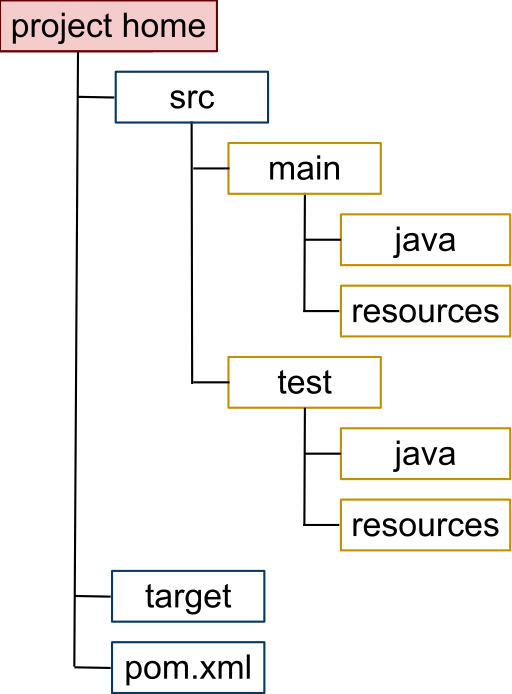
\includegraphics[scale=0.3]{figures/1}
\end{center}
\begin{compactitem}
\item project home	- Contains the pom.xml and all subdirectories.
\item src/main/java - Contains the deliverable Java sourcecode for the project.
\item src/main/resources - Contains the deliverable resources for the project, such as property files.
\item src/test/java - Contains the testing sourcecode (JUnit test cases, for example) for the project.
\item src/test/resources - Contains resources necessary for testing.
\end{compactitem}

A Project Object Model (POM) contains all the configuration for a
single project. General configuration covers the project's name, its
owner and its dependencies on other projects. 

To obtain an executable version of the application, the project must be
compiled, built and exported (as a .jar file, usually) with a
correctly configured classpath to all the classes of the
external libraries used in the project (i.e., dependencies) )as well 
as the entry point class (i.e., the Main class). It is a
good practice to also test the application before using it.

Doing this manually every time would be cumbersome, thus in this
lab we will use Maven to automatize the build process.
Maven follows a build lifecycle when building the project. Build
lifecycle is a list of phases that must be executed sequentially to
build the project.

\begin{compactitem}
\item validate
\item generate-sources
\item process-sources
\item generate-resources
\item process-resources
\item compile
\item process-test-sources
\item process-test-resources
\item test-compile
\item test
\item package
\item install
\item deploy
\end{compactitem}

When invoking a maven build you may specify any of the phases as a
goal of the build. Maven would then execute sequentially all phases
before the goal and the goal phase itself. For example, if you specify
\texttt{compile} as a goal, phases \texttt{validate},
\texttt{generate-sources}, \texttt{process-sources},
\texttt{generate-resources}, \texttt{process-resources},
\texttt{compile} are going to be executed.
You can also customize individual phases of the build process. This is
implemented using plugins specified in the pom.xml file. For example,
one can configure the compiler-plugin to use Java version 1.7 for
compilation.

A central feature in Maven is dependency management. If you are
developing a project that uses external libraries you do not need to
provide them together with your project. It is enough to specify the
dependency in the pom.xml file and  during the build Maven will
automatically download the dependency and in turn, all the
dependencies that the dependency itself needs (called transitive
dependencies).

There are two types of repositories where maven searches for
dependencies: local and remote. Maven automatically creates a local
repository on your machine (usually on the .m2 folder) that contains
the cache of your downloaded dependencies, as well as the
temporary builds of projects that you manage with maven.

Maven provides a remote ``Central Repository''  that is used by default to search
for dependencies, but other repositories can be specified and used.

Maven's is able to find dependencies based on the coordinates (Group
ID and Artifact ID) that identify individual software libraries or
modules.

\subsection{Maven Plugin for Eclipse (m2e)}

Maven Integration for Eclipse, named `m2e', provides the following features:
\begin{compactitem}
\item Launching Maven builds from within Eclipse
\item Dependency management for Eclipse build path based on Maven's pom.xml
\item Resolving Maven dependencies from the Eclipse workspace without installing to local Maven repository
\item Automatic downloading of the required dependencies from the remote Maven repositories
\item Wizards for creating new Maven projects, pom.xml and to enable Maven support on plain Java project
\item Quick search for dependencies in Maven remote repositories
\item Quick fixes in the Java editor for looking up required dependencies/jars by the class or package name
\end{compactitem}

\subsection{Install Maven}
Eclipse 4.4.2 comes with installation of m2e, so the installation is
not needed. If you are using an older version of Eclipse (not
recommended) you can install last m2e release by using the following
update site from within Eclipse: 

\url{http://download.eclipse.org/technology/m2e/releases/}

Perform following steps:
\begin{compactitem}
\item To to Help > Install New Software
\item Copy the above URL into the topmost textbox
\item Click on add and give it a name
\item After clicking OK, the list below should contain ''Maven Integration for Eclipse``
\item Check it
\item Click Next, Next, Accept, Finish
\end{compactitem}

\section{Create a Maven project}
Maven provides project templates called archetypes. The archetype
specify the type of project we want to create. Each archetype
corresponds to a particular type of application we want to develop.

The archetype generation need:
\begin{compactitem}
\item \textbf{Archetype}: kind of project we want to create
\item \textbf{Group ID}: Explanationar Id when my project includes multiple artifacts
\item \textbf{Artifact ID}: output of project web application (WAR) Enterprise application (EAR) Simple Java application (Jar)
\item \textbf{Version}: 1.0 we are developing at the end we can release
\item \textbf{Package}: where we want to put the source code
\end{compactitem}

Archetype defines:
\begin{compactitem}
\item Folder structure
\item pom.xml
\end{compactitem}

To create a maven project:
\begin{compactitem}
\item Click File $>$ New $>$ Project ...
\item Choose Maven project
\item Click Next and choose \texttt{maven-archetype-quickstart} as
  shown in the figure:
\begin{center}
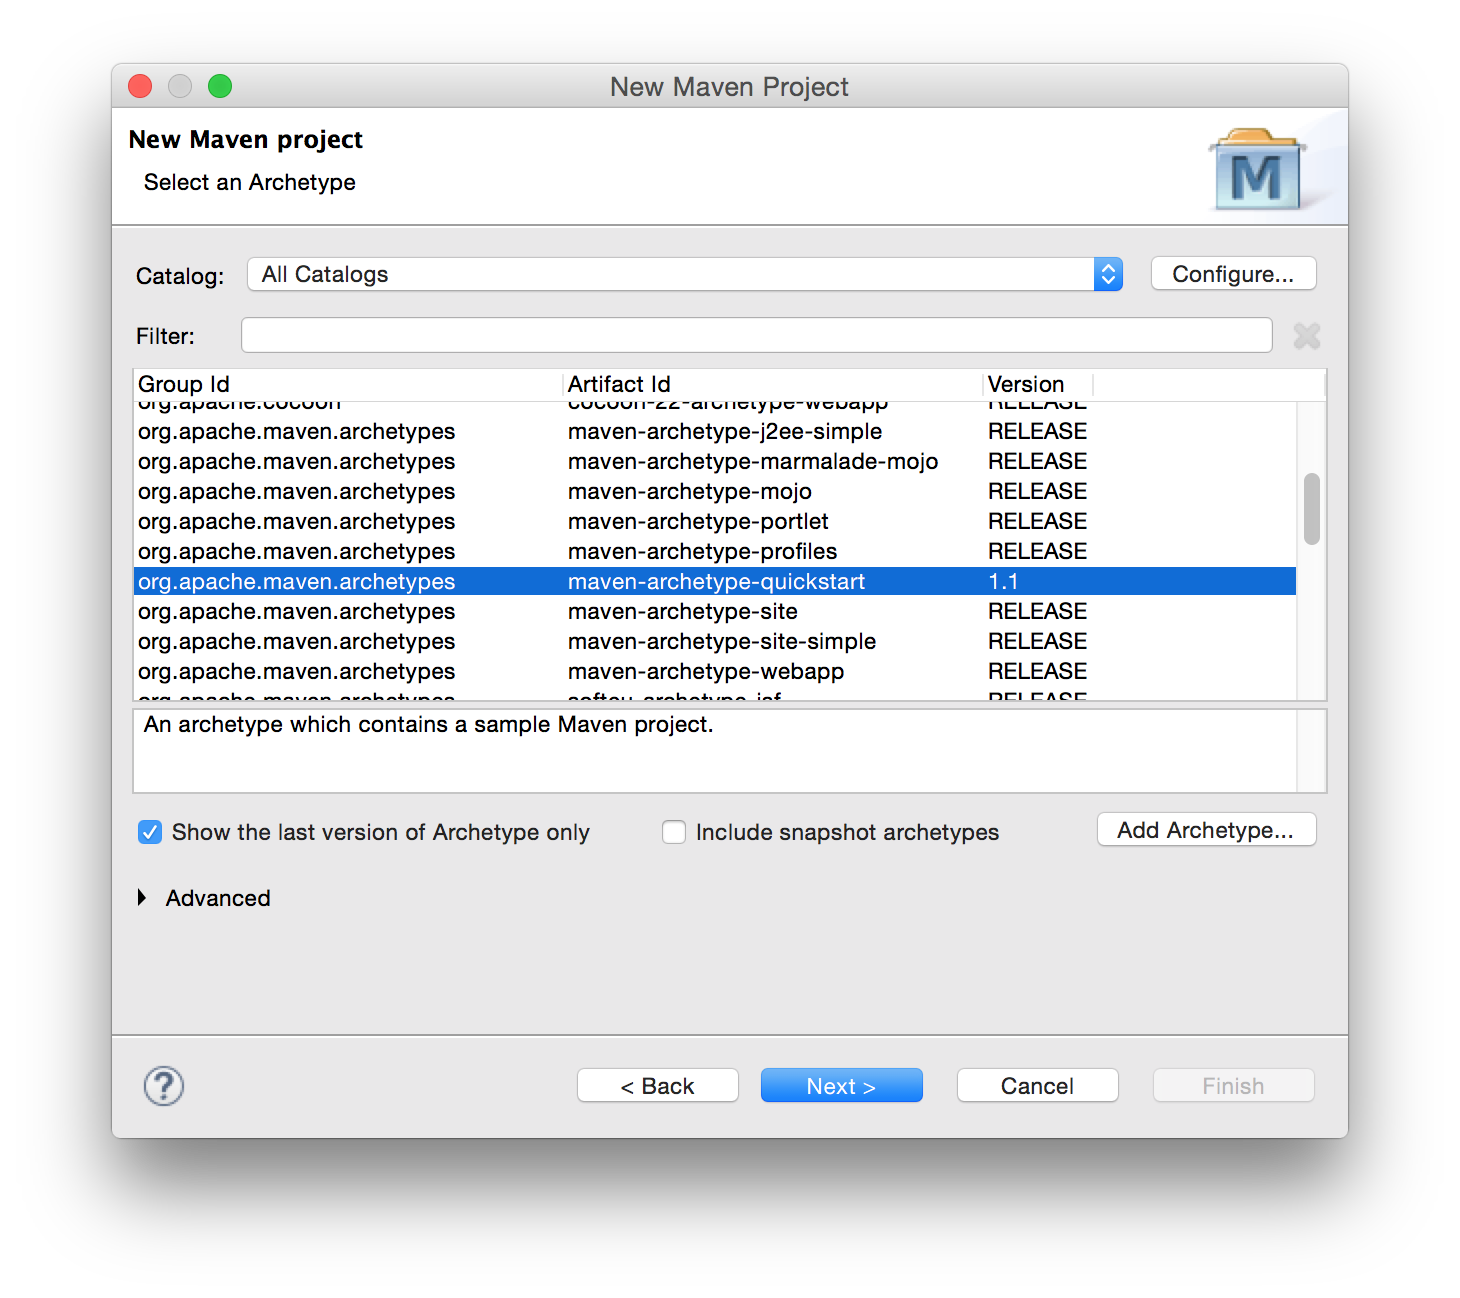
\includegraphics[scale=0.5]{figures/2}
\end{center}
\item Click Next. Set group ID to it.polimi.ingsw and artifact ID
  to cg\_*number* were *number* is the number of your group. You will
  be informed about your number by the lab responsibles. Figures show
  the example for project cg\_1.
\begin{center}
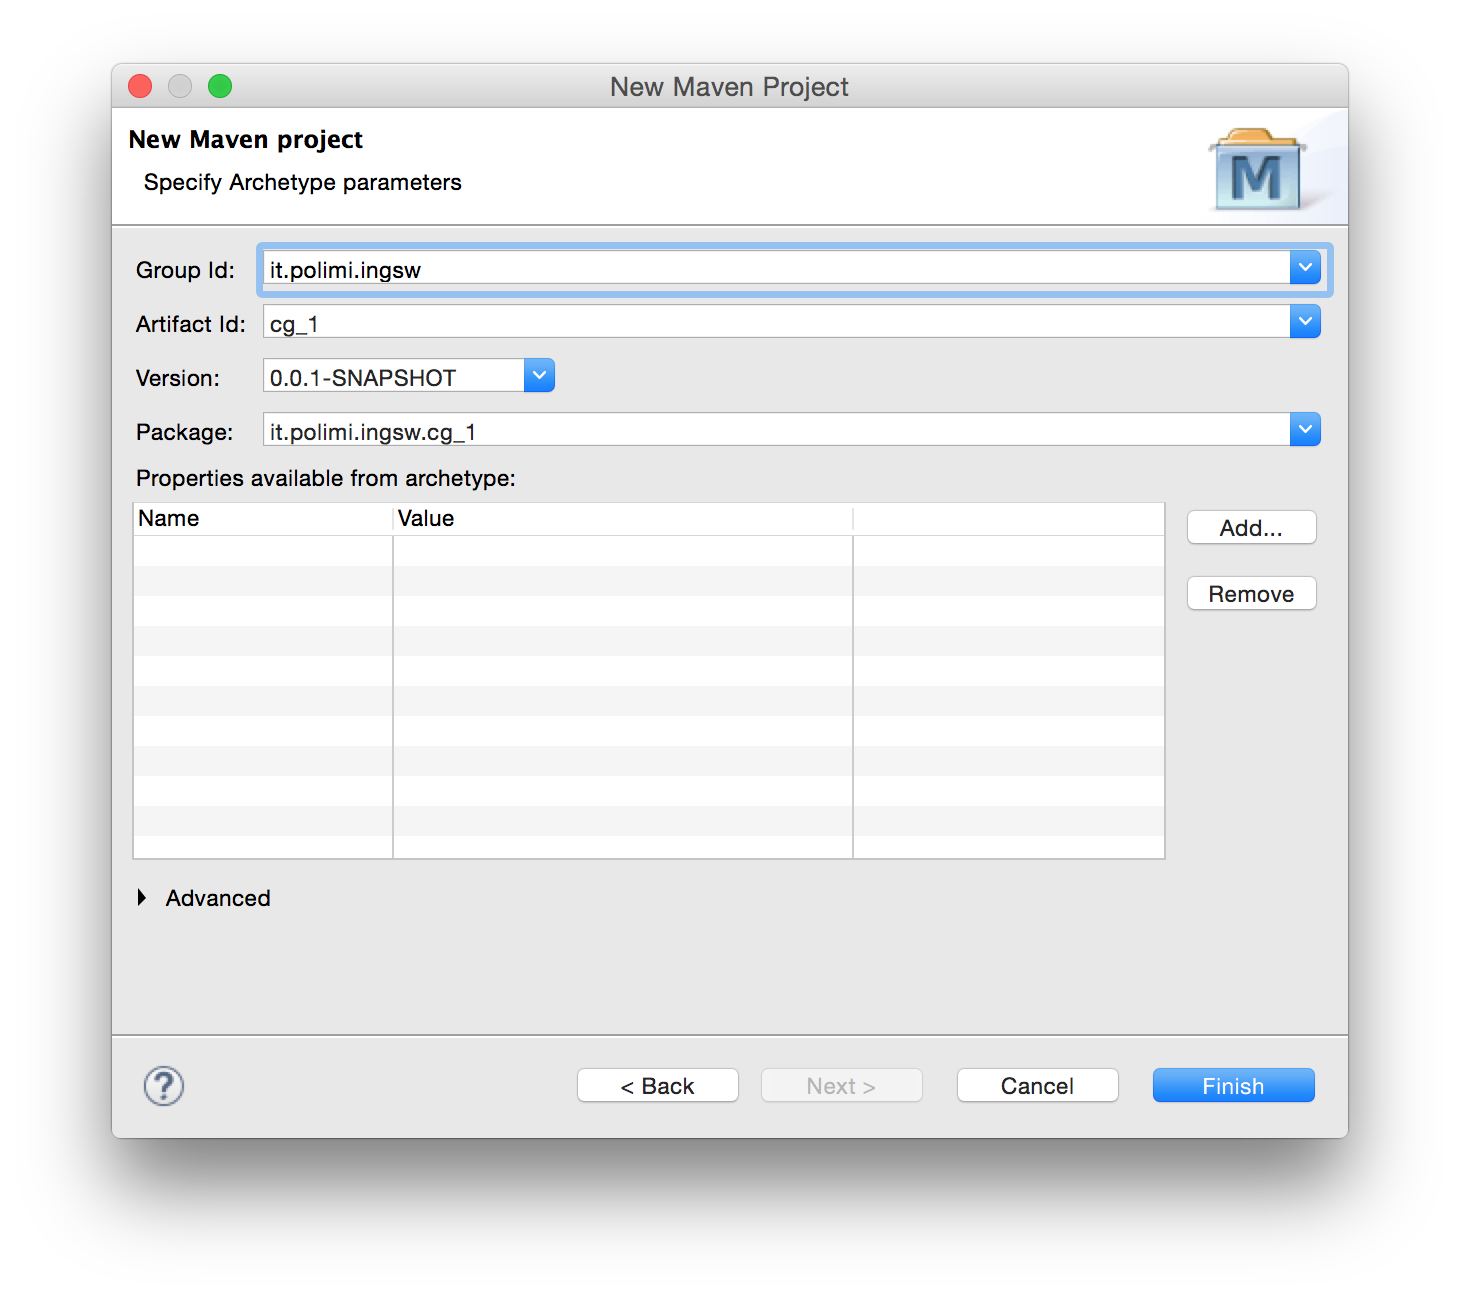
\includegraphics[scale=0.5]{figures/3}
\end{center}
\item Click finish and wait for the Maven to create the project. You
  should see the following structure of the project 
\begin{center}
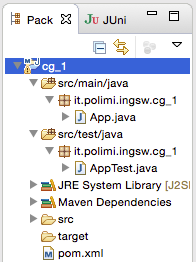
\includegraphics[scale=0.5]{figures/4}
\end{center}
\item Open pom.xml file (shown in the Package explorer on the left),
  choose the pom.xml tab in the lower part of the window and change it
  to match the pom.xml file shown below. Keep in mind to replace
  *number* with your appropriate number.
\end{compactitem}



\section{Pom.xml file for the lab}

\begin{lstlisting}
<project xmlns="http://maven.apache.org/POM/4.0.0" xmlns:xsi="http://www.w3.org/2001/XMLSchema-instance" xsi:schemaLocation="http://maven.apache.org/POM/4.0.0 http://maven.apache.org/xsd/maven-4.0.0.xsd">
  <modelVersion>4.0.0</modelVersion>
  <groupId>it.polimi.ingsw</groupId> 
  <artifactId>cg_*number*</artifactId> 
  <version>0.0.1-SNAPSHOT</version>
  <name>cg_*number*</name>
  <properties>
     <project.build.sourceEncoding>UTF-8</project.build.sourceEncoding>
     <sonar.language>java</sonar.language>
     <sonar.host.url> http://localhost:9000/ </sonar.host.url>
  </properties>
  <description>Prova Finale Ingegneria del software</description>
  <dependencies>
    <dependency>
      <groupId>junit</groupId>
      <artifactId>junit</artifactId>
      <version>4.12</version>
      <scope>test</scope>
    </dependency>
  </dependencies>
  <build>
    <plugins>
      <plugin>
        <groupId>org.apache.maven.plugins</groupId>
        <artifactId>maven-compiler-plugin</artifactId>
        <version>3.2</version>
        <configuration>
          <source>1.7</source>
          <target>1.7</target>
        </configuration>
      </plugin>
      <plugin>
	<groupId>org.jacoco</groupId>
	<artifactId>jacoco-maven-plugin</artifactId>
	<version>0.5.5.201112152213</version>
	<configuration>
	  <destFile>target/jacoco.exec</destFile>
	  <dataFile>target/jacoco.exec</dataFile>
	</configuration>
	<executions>
	  <execution>
	    <id>jacoco-initialize</id>
	    <goals>
	      <goal>prepare-agent</goal>
	    </goals>
	  </execution>
	  <execution>
	    <id>jacoco-site</id>
	    <phase>package</phase>
	    <goals>
	      <goal>report</goal>
	    </goals>
	  </execution>
	</executions>
      </plugin>
    </plugins>
  </build>
</project>
\end{lstlisting}


\end{document}




